% !TEX root = ../main.tex
\section{Evaluation of Graphical Password Schemes} \label{sec:evaluation}
	
  Authentication with text-based passwords are a traditional approach, but as a result of limitations of recalling text-based passwords, users choose weaker passwords. Graphical passwords came as an alternative solution for overcoming the limitations of text-based passwords because the graphical memory of humans is particularly well-suited to remember graphical information \cite{DeAngeli}. The problem with many graphical password schemes is that they often promise improved password memorability and thus usability, and at the same time improve the security \cite{Biddle}. The trade-off between usability and security is illustrated in Figure~\ref{fig:usabilitysecurity}. The observed trade-off between usability and security are two aspects important to understand while reviewing the literature of graphical passwords.

  	\begin{figure}[H]
  		\centering
  		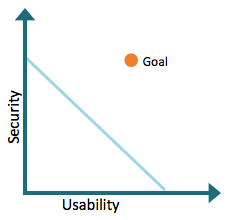
\includegraphics[width=0.40\textwidth]{pics/review/tradeoff.png}
  		\caption{Tradeoff between usability and security}
  		\label{fig:usabilitysecurity}
  	\end{figure}

  \subsection{Usability and Memorability} \label{sec:usability}

    An interesting question is what types of graphical password users find memorable. One of the factors supporting users to remember their selected password relates to the usability of the password scheme. What grants a graphical password high usability and what is the effect of having high usability? This section will look at different graphical password schemes focusing on the usability of the scheme. 

    Deja Vu was one of the graphical password schemes created in order to be easy to remember, but at the same time being hard to reuse and share as a result of the random art used. When {\it Deja Vu} was first proposed, the creators conducted a user study showing that 90\% of all participants succeeded the authentication phase using Deja Vu. On the other side, the creators also revealed that only 70\% managed to pass the authentication process by using text-based passwords and PIN codes \cite{DejaVu}. The difference in success rate is an example of users tending to have a higher success rate remembering graphical password over text-based passwords and PIN codes. 

    One of the first graphical password schemes, {\it DAS} \cite{Jermyn}, offered a theoretical space comparable with text-based passwords. Based on cognitive studies of visual information, Oorschot and Thorpe \cite{Thorpe1} investigated the practical password space of the graphical password scheme {\it DAS} \cite{Jermyn}. They found that the password space in practice in {\it DAS} represented an average length less than or equal to the length of 8 on a 5$\times$5 grid. 

    Other researchers have revealed that users tend to draw symmetric images with few pen strokes as well as placing their drawings in the center of the grid. The researchers behind {\it Background Draw A Secret}\cite{BDAS} tried to avoid users placing their drawings in a predictable way and by adding a background image to avoid the predictable behavior. The attached background image resulted in a reduced amount of symmetry within the selected passwords and helped the users make longer passwords that were similarly memorable as for {\it DAS}.

    Davis \cite{Davis} did a comparison of the memorability between the graphical password scheme {\it Face} (a light version of the {\it PassFaces}) and {\it Story}. The result reported that users had more difficulties remembering the Story password, resulting in a success rate of  85\%. The low success rate was observed because the users had to remember the correct sequence of the images, rather than remembering the images in an arbitrary sequence. 

    When considering usability, we can evaluate the graphical layout of a graphical password scheme to see if the visual elements impact the user's choice of passwords. Ullenbeck et al. \cite{Uellenbeck} considered the Android Unlock patterns and investigated whether a change in the graphical layout would impact the security and usability. The original Android Pattern Lock uses a sequence of dots connected in a 3$\times$3 grid of nodes. Instead of only analyzing the original scheme, they rearranged the points into four separate positions and analyzed patterns created by users for all four rearrangements. The results proved that the number of unique patterns created was doubled by rearranging the points, hence reduced the bias found in the original position of the nodes. However, they did not only remove some of the bias from the original grid, but also introduced new ones. One of the rearrangements was a random approach. Unfortunately, this random arrangement of nodes looked like the mathematical {\it delta}, an association element that was recognized by several of the participants. The random arrangement scored the worst entropy seeing as many of the users selected the same pattern. People are good at recognizing patterns and using association elements. It would not be surprising if users found similar results in other rearrangements of the grid if it had a shape similar to other symbols or association elements.

    Wiedenbeck et al. \cite{Wiedenbeck1, Wiedenbeck2, Wiedenbeck3} conducted three lab-based user studies on the graphical password scheme {\it PassPoint}. The results determined that the participants needed an average time of 63 seconds to create their password, and an additional average time of 171 seconds in training time to remember the created password. The login time took between 9 and 19 seconds on average. The time spent highlights the importance of research on usability and memorability when considering graphical password schemes. The factors that grant a password scheme high usability can be determined by looking at the average creation time, time to remember the password, as well as time used in the login phase. 

    It is still a problem that published research on graphical passwords focusing on usability are conducted with a pen and paper approach, raising a question about the results’ validity. One problem may be that many graphical passwords are not implemented, but rather theoretical and visual suggestions. There is still a need for further research on graphical passwords in their actual intended environment of use.

	\subsection{Security} \label{sec:security}

    In knowledge-based authentication, e.g. {\it something you know}, we classify attacks into two general categories: guessing and capturing attacks. In a guessing attack, the adversary must search through the entire password space; this is often referred to as a brute force attack. A brute force attack validates all possible combinations, making such an attack highly time-consuming. If an attacker has some knowledge of the user or the user’s password habits, the attacker would be able to predict the user's password by avoiding searching through the whole password space. Such a reduction in the password space is a reduction in the overall security of the scheme. When managing to reduce the search space, this type of attack is often referred to as a dictionary attack. When talking about capturing attacks, the attackers can directly obtain the passwords by observing the authentication process. One of the known capturing attacks on graphical passwords is shoulder surfing where an attacker is able to observe a user's password as a cause of a visual presence.

    When selecting a password, many users select a password that connects to them as a person or to something they know. By using this strategy in the process of creating a password, there will be a lower probability of forgetting the password because the password is something you already know. When using such an approach, it is more likely that the person remembers the password, while at the same time helping an attacker to be able to guess the selected password quickly. There is a tradeoff between what is possible to remember and what is secure enough to use; attackers utilize our predictable behavior. A password created using this predictable behavior is called a biased password. A bias is a prejudice in favor of or against one thing, person, or group compared with another, usually in a way that influences a person's choice of action.

    Jermyn et al. \cite{Jermyn} evaluated the security of the graphical password scheme {\it DAS}. One of the statements is that the users do not utilize a uniform distribution of the possible passwords by using Klein's study \cite{UnixPasswords} as an argument. The fact that users do not pick passwords uniformly is no itself a sufficient statement to make a guessing attack successful. They try to cover the possibility of an attacker making a successful attack by making their scheme more complex. The results revealed that the generated passwords were significantly harder to crack in practice than textual passwords. The problem with the conducted tests was that they used computer generated passwords that do not achieve the same validity as user-selected passwords. Neither did they analyze the security of {\it DAS} by including human factors that earlier have been reported to introduce bias in the password selection process.

    Why do users select the passwords they do, and what strategy do they use in the creation process? Davis et al.\cite{Davis} evaluated the security of the graphical password scheme {\it Passfaces}. They found that there was a bias introduced by people's demographics and background. The users tended to choose faces that they liked (their subjective meaning of beauty and attractiveness) and faces they could compare to themselves. The results revealed that with sufficient knowledge of the gender and race of the user, it would be possible to perform a dictionary attack to guess user-selected passwords in the {\it PassFace} scheme. If the user were male, 10\% of the passwords could easily be guessed on the first or second attempt. Similarly, if the race of the user was known to be Asian and his/her gender was also known, then 10\% of the passwords could be guessed within the first six attempts. The result indicated that graphical passwords selected by users were heavily biased. The researchers concluded that Passfaces was insecure due to the observed bias in the selection of passwords. 

    Dirik et al. \cite{Dirik} conducted an experiment by modeling users choice in the graphical password scheme {\it PassPoints}. The aim of the study was to test whether it would be possible to build a dictionary attack based on a user's choice of clicking points. In this study, they predefined two different images with a different level of salient points. The researchers reported that they could recover 61\% of a user's selection of clicking points by searching through a smaller password space based on an analysis of collected click-points. The {\it PassPoints} scheme provides user-chosen images, but the aim of this study was to investigate whether it was possible to predict user's passwords using a dictionary attack on images after collected data. They observed a slight difference in two out of three images picked by the researchers. The images including few salient points were being stated as less insecure. Since the {\it PassPoints} scheme enabled user-selected images, the security would rely on the image and clicking points selected by the user, and not the actual scheme itself. The results can not solely state that using {\it PassPoints} is insecure, but rather highlight the importance of considering the human factors in security as it can influence the overall security of the scheme. The same year, another research group published results on security of {\it Passpoints} by using two separate research methods  \cite{Thorpe2}. They conducted a user study, as well as a theoretical study image-processing tool, to test whether an attack on the {\it PassPoints} scheme was possible. They provided empirical evidence that attractive points, e.g. hot-spots, do exist in images. The results from the most efficient attack were generated by harvesting passwords from users to attack other targets. The probability of the guessing attack showed that 36\% of the passwords selected by users ended up being guessed within $2^{31}$ guesses and 12\% could be guessed within $2^{16}$ guesses. The results from the simulated attack using image-processing were slightly less efficient, but they still managed to prove that an attack on graphical passwords is possible.
    
    One of the first large-scale studies on the Android Pattern Lock \cite{Uellenbeck} stated that the entropy of a pattern is lower than its theoretical entropy. The research group compared the security offered by the Android Pattern Lock to be less than the security of a randomly assigned three-digit PIN for guessing 20\% of all passwords. In the same research, a Markov model based on collected passwords was built. The patterns created was categorized as offensive and defensive patterns as a result of their research design. They set up a game asking all respondents to create a defensive pattern protecting a possible award, as well as creating offensive patterns used for guessing other participants' defensive patterns. The results showed that it was possible to guess a user's choice of patterns. Within ten guesses, they could guess approximately 4\% of the defensive patterns and approximately 7\% of the offensive patterns. When increasing the number of guesses to 30 attempts, they managed to guess approximately 9\% of the defensive patterns and approximately 19\% of the offensive patterns. If we look further into the Android Unlock Pattern, the scheme has roughly 400.000 possible valid combinations of patterns. From a theoretical point of view, such theoretical password spaces are comparable to the security of a 5-digit randomly assigned PIN. The researchers’ evaluation of user-chosen patterns explains that they only have an estimated entropy slightly lower than a 3-digit randomly assigned PIN. Another interesting discovery by the researchers is that around 10\% of all users use less than 190 patterns, while less than 300 patterns capture around 50\% of the whole test popluation. This result is an indication of the theoretical password space not being a representative number when quantifying the security of a password scheme. We should rather look at the password space in practice, e.g. passwords that are used and memorized by users.

    Psychology studies have recognized humans' superior memory for recognizing and recalling visual information. This observation supports the statement that users can remember more complicated graphical password from a larger password space than an alphanumeric password. Based on this assumption, the attacker needs to build a bigger and more complex dictionary and spend more time achieving the same success rate as for textual passwords. A clever attacker would narrow down the password space and prioritize guesses to pictures that people are likely to choose. The images that are selected are liable to be the images that users are likely to recall. To understand how an attacker might take advantage of human password choices, psychological studies on humans' visual memory are crucial to comprehend.
